\chapter{\label{searchcw}Searching for continuous gravitational waves}
%%%%

%--------------------
% introduce problems in searching for CW
%---------------------
\glspl{CW} have
particular challenges when it comes to their detection.  \glspl{CW} are long
duration, this means that they would be observed for the entirety of a
detectors observing run.  The signals also have an intrinsically small
amplitude which is below the noise floor of current ground based detectors such
as \gls{LIGO}.  This means that for a detection, the entire observing
run's data will be needed to
accumulate enough \gls{SNR} for a signal to be observed.  Given that \gls{LIGO}
samples at $\sim 16$ kHz (generally downsampled to $\sim 4$ kHz) this leaves a
huge amount of data ($\mathcal{O}(2)$ TB for one year at 16kHz) which needs to be searched through.  As will be described in Sec.~\ref{searchcw:search}, this means that a large amount of computational resources is required to perform a search for \gls{CW}.
For some types of search the parameter space can also be very large, this only
adds to the computational time and in some cases makes the search
infeasible.

%---------------------
% Describe this chapter 
%--------------------------
Whilst I have described the potential sources a \gls{CW} signal and its approximate
signal type in Sec.~\ref{intro:sources:cw}, to perform a search the we need to understand the
intrinsic waveform of the signal and the observed waveform at a detector.  In 
Sec.~\ref{searchcw:model} we will go into more
detail on the \gls{CW} signal model. In Sec.~\ref{searchcw:bayes} we introduce Bayesian techniques which can be used in many analyses. The \gls{CW} signal model and Bayesian techniques is then used in various search methods for
\gls{CW} signals, where I will overview a subset of current searches in
Sec.~\ref{searchcw:search}.

%%%%%
%%%%%
\section{\label{searchcw:model}Continuous signal model}
%%%%
%%%%

The model of a \gls{GW} signal from a rapidly rotating neutron star is relatively simple, it is intrinsically a
quasi-sinusoidal signal, meaning that it is a sinusoid with a slowly
varying frequency. This indicates that as the neutron stars rotational frequency decreases (spins down) it is losing energy. The rate at which the star loses energy is generally characterised by the braking index defined by
\begin{equation}
	n = \frac{f_{\rm{rot}} \ddot{f_{\rm{rot}}}}{\dot{f_{\rm{rot}}}^2},
\end{equation}
where $f_{\rm{rot}}$ is the rotational frequency of the neutron star \citep{dearaujo2016GravitationalWaves}.
There are a number of potential reasons for the spin down, including: the energy loss to \gls{GW}, which should have a braking index of 5 \citep{dearaujo2016GravitationalWaves} and magnetic braking which gives a braking index of 3 \citep{dearaujo2016GravitationalWaves}.

The parameters of each neutron star can be split into two sections: the Doppler components
($\alpha,\delta,{\bm f}$) and its amplitude components ($\psi,\phi_0, \iota,
h_0, \theta$). This ignores any orbital parameters which would be present if the
star was in a binary systems. The Doppler parameters are defined as follows: the sky positions
$\alpha$ and $\delta$ refer to the right ascension and declination of the source. The frequency ${\bm f}$ refers to
the \gls{GW} source frequency and its spin derivatives.  The parameters $\psi$,
$\phi_0$ and $h_0 $ are the \gls{GW} polarisation, initial phase and amplitude
respectively.  The inclination angle $\iota$ is the angle between a vector pointing towards the source and the rotation axis of the source. 
Finally, $\theta$ is the `wobble angle' or the angle between the rotation axis and the
symmetry axis of the neutron star.

The definition of the \gls{GW} from a neutron star given here follows that in
\citep{riles2017RecentSearches,schutz1998DataAnalysis,dupuis2005BayesianEstimation}.
The amplitude of the \gls{GW} is defined in Eq.~\ref{intro:detector:strain_2}, however I will redefine it here
%
\begin{equation}
\label{searchcw:model:amplitude}
h(t) = F_{+}h_{+}(t) + F_{\times}h_{\times}(t),
\end{equation}
%
where $h_{+},h_{\times}$ are the plus and cross polarisation functions as defined in
Eq.\ref{intro:gw:gravwave}, and $F_{+},F_{\times}$ are the antenna pattern
functions  defined in Eq.\ref{intro:detector:response:polarisations}. The plus a cross polarisation functions are defined by
%
\begin{equation}
\label{intro:cw:amplitudes}
    \begin{split}
        h_{+}(t) &=  h_0 \frac{1 + \cos^2{(\iota)}}{2}\cos{\left(\Phi(t)\right)} \\
        h_{\times}(t) &= h_0  \cos{(\iota)} \sin{\left( \Phi(t)\right) }, \\
    \end{split}
\end{equation}
%
where $h_0$ is the \gls{GW} amplitude, $\iota$ is the inclination angle of the source and $\Phi(t)$ is the phase of the \gls{GW}. 
Here we assume the wobble angle $\theta$ is assumed to be small,
however this is included in the derivation in \citep{schutz1998DataAnalysis}.
The phase of the wave $\Phi(t_{{\rm SSB}})$ at the \gls{SSB} can be defined as
%
\begin{equation}
\label{searchcw:model:phase}
    \Phi(t_{{\rm SSB}}) = \phi_0 + 2\pi\left[ f_0(t_{{\rm SSB}} - t_0) + \frac{1}{2} \dot{f_0} (t_{{\rm SSB}} - t_0)^2 + .....\right] .
\end{equation}
%
This consists of an initial phase $\phi_0$ which is the phase at time $t_0$,
the frequency of the \gls{GW} signal $f_0$ and its derivative ${\dot{f}}$ measured at
time $t_0$. The time at the \gls{SSB} $t_{{\rm SSB}}$ can be
transformed to the time $t$ at the detector by
%
\begin{equation}
	\label{searchcw:model:ssbtime}
t_{{\rm SSB}} = t + \frac{\mathbf{r}_d \cdot \mathbf{n}}{c} + \delta_t,
\end{equation}
%
where $c$ is the speed of light, $\mathbf{r}_d$ is the position of the detector with reference to the
\gls{SSB}, $\mathbf{n}$ is a unit vector in the direction of the source. The factor $\mathbf{r}_d \cdot \mathbf{n}/c$ takes into account the Doppler shift of the
signal due to the movement of the detector, i.e. as the earth rotates on its axis and
orbits the sun. The factor $\delta_t$ take into account extra
corrections from the Einstein and Shapiro delay
\citep{taylor1992PulsarTiming}. Einstein delay accounts for the time dilation and and gravitational redshift due to the Sun. Shapiro delay originates from the extra time a signal takes to pass through the gravitational potential of the Sun. \joe{need to properly understadn difference nbetween these two}The amplitude
$h_0$ in Eq.~\ref{intro:cw:amplitudes} is defined by
%
\begin{equation}
    h_0 = \frac{4 \pi^2 G}{c^4} \frac{\epsilon I_{zz} f^2}{r},
\end{equation}
%
where $G$ is the gravitational constant, $\epsilon$ is the ellipticity of the star, $f$
is the \gls{GW} frequency, $r$ is the distance to the star and $I_{zz}$ is the
moment of inertia with respect to the rotation axis $z$.  The ellipticity $\epsilon$ is a measure of the distortion of the star around its rotation axis and is defined in Eq.~\ref{intro:source:cw:ellipticity}, however I will redefine it here
%
\begin{equation}
    \epsilon = \frac{I_{xx} - I_{yy}}{I_{zz}},
\end{equation}
%
where $I_{xx}, I_{yy}$ and $I_{zz}$ are the moments of inertia for each axis.

In Eq.~\ref{searchcw:model:amplitude}, $F_+(t)$ and $F_{\times}(t)$ are the antenna pattern
functions of the detector.  These describe how sensitive a detector is to a
particular location on the sky and are described in Sec.~\ref{intro:detector:response} where the response to
sky location is shown in Fig.~\ref{intro:detector:response:polarisations}.  In \citep{schutz1998DataAnalysis} these are defined more completely
%
\begin{equation}
\label{intro:cw:antenna}
\begin{split}
F_{+}(t) &= \sin{\zeta}[a(t)\cos{(2\psi)} + b(t)\sin{(2\psi)}], \\
F_{\times}(t) &= \sin{\zeta}[b(t) \cos{(2\psi)} - a(t)\sin{(2\psi)}],
\end{split}
\end{equation}
%
where $\zeta$ is the angle between the arms of the detectors, $\psi$ is the
polarisation angle of the \gls{GW} and $a(t)$ and $b(t)$ are defined in
\citep{schutz1998DataAnalysis} and relate the sky location to the orientation
of the detector at a given time.  A full derivation of this can be found in
\citep{schutz1998DataAnalysis} where each of these terms are expanded.
Equations \ref{searchcw:model:amplitude} - \ref{intro:cw:antenna} then describe the amplitude and phase evolution of a
signal at a given detector location and orientation.



%%%%%%%%%%%%%
%%%%%%%%%%%%%%%
%%%%%%%%%%%%%%%%
\section{\label{searchcw:prob} Bayes Theorem}
%%%%%%%%%%%%%%%
%%%%%%%%%%%%%%%%
%%%%%%%%%%%%%%%%%

A key part in understanding the different methods used to search for
\gls{GW} or many other data analysis problems, is understanding probability
and statistics.  This gives us understanding of the random processes
underlying all measured quantities.  Whilst there are generally two approaches
to statistics: Frequentist and Bayesian, here I will focus on the Bayesian
approach.  

%%%%%%%%%%%%%
%%%%%%%%%%%%%
\subsection{\label{searchcw:prob:basic}Basic probability}
%%%%%%%%%%%%%%
%%%%%%%%%%%%%%

Initially I will define some basic concepts of probability.  We can define the
probability of some event $A$ as $p(A)$ where probabilities lie in the range $0 \leq p(A)
\leq 1$ and some other event $B$ which has a probability $p(B)$ and
which lies in the range $0 \leq p(B) \leq 1$.

\begin{description}
	\item [Union]
	A union is the probability of either event $A$ happening or event $B$ happening. This is written as, $p(A \cup B)$.
	
	\item [Intersection]
	An intersection is then the probability that both and event $A$ and an event $B$ happens. This is written as $p(A \cap B)$.
	
	\item [Independent and dependent Events]
	If the events $A$ and $B$ are independent, i.e. the event $A$ does not affect the outcome of event $B$, then
	\begin{equation}
	p(A \cap B) = p(A)p(B).
	\end{equation}
	However, if the event $A$ is dependent on event $B$, i.e. the event $A$ affects event $B$ or vice versa, then the joint probability of both events is
	\begin{equation}
	\label{searchcw:prob:dependentevent}
	p(A \cap B) = p(A)p(B \mid A) = p(B)p(A \mid B).
	\end{equation}
	Here $p(B \mid A)$ means the probability of event $B$ given an event $A$.
	
	\item [Conditional probability]
	Conditional probability arises from situations where one event $A$ affects the event $B$.
	The definition of this arises from the the dependent events defined above in Eq.~\ref{searchcw:prob:dependentevent}
	\begin{equation}
	p(A \mid B) = \frac{p(A \cap B)}{p(B)}.
	\end{equation}
	
	\item [Bayes Theorem]
	Bayes theorem can then be defined using conditional probabilities. i.e we can use
	\begin{equation}
	p(A \mid B) = \frac{p(A \cap B)}{p(B)} \quad \rm{and} \quad p(B \mid A) = \frac{p(A \cap B)}{p(A)}
	\end{equation}
	such that
	\begin{equation}
	p(B)p(A \mid B) = p(A)p(B \mid A)
	\end{equation}
	and this is rearranged to Bayes theorem
	\begin{equation}
	\label{searchcw:prob:bayes}
	p(A \mid B) = \frac{p(A)p(B \mid A)}{p(B)}
	\end{equation}
	
\end{description}

%%%%%%%%%%%%%%%%%
%%%%%%%%%%%%%%%%%%
\subsection{\label{searchcw:bayes}Bayesian Inference}
%%%%%%%%%%%%%%%%%%%
%%%%%%%%%%%%%%%

We can take Bayes theorem from Sec.~\ref{searchcw:prob:basic} and apply it to a
problem which involves inferring the parameters from some model. Here we can
relabel the events $A$ and $B$ with the data ${\bm d}$ and the parameters ${\bm
\theta}$ of some model $I$.  Equation \ref{searchcw:prob:bayes} then becomes
%
\begin{equation}
\label{searchcw:bayes:bayes}
p({\bm \theta} \mid {\bm d}, I) = \frac{p({\bm \theta}, I)p({\bm d} \mid {\bm \theta}, I)}{p({\bm d} \mid I)}
\end{equation}
%
where each of the components are assigned names: $p({\bm \theta} \mid {\bm d})$
is the posterior distribution, $p({\bm \theta})$ is the prior distribution,
$p({\bm d} \mid {\bm \theta})$ is the likelihood, and $p({\bm d})$ is the
Bayesian Evidence.

\begin{description}
	\item [Posterior]
        The posterior distribution describes the probability of a parameter
${\bm \theta}$ in some model $I$ given some data $d$. For many problems this is
the distribution which is most useful as it informs you how likely any set of
parameters from your model are given some observation.
	
        \item [Prior] The Prior distribution is a key part of Bayesian
statistics which describes the distribution of the parameters ${\bm \theta}$ given the model $I$. This should reflect any beliefs about the parameters $\theta$ prior to the observations.
	
        \item [Likelihood] The likelihood is where the observation is included
in the calculation. This tells you how probable it is to get the observed data
$d$ given the model $I$ with the set of parameters $\theta$. 
	
        \item [Bayesian Evidence] This is the probability of the data itself
given the choice of model. This is found by integrating the likelihood over all
possible values of ${\bm \theta}$ weighting them by our prior belief of that
value of ${\bm \theta}$. This is also known as the marginal
likelihood and is defined by,
	%
        \begin{equation} \label{searchcw:bayes:evidence} 
            p({\bm d} \mid I) = \int p({\bm \theta}, I)p({\bm d} \mid {\bm \theta}, I) d{\bm \theta}.
        \end{equation} 
\end{description}

Bayes theorem then gives a description of the probability distribution of some
parameters in a model given some observation.  Often when using Bayesian
statistics the aim is to find the posterior distribution of parameters.  There are
very few cases where this can be calculated analytically, therefore, numerical
methods are often used to find the posterior.  This
can be difficult to calculate numerically especially in problems where the
parameter space has many dimensions.  The most difficult part to calculate is
the Bayesian Evidence in Eq.~\ref{searchcw:bayes:evidence} which involves calculating an
integral over all possible parameters.  However, if you are only interested in the posterior there is a way around having
to calculate this.  For any given model $I$, the Bayesian Evidence $p({\bm d}\mid I)$ is
independent of any parameters ${\bm \theta}$ in
Eq.~\ref{searchcw:bayes:bayes} and depends only on the model $I$.
The Bayesian Evidence is then just a normalisation factor for the posterior
distribution.  When different models are not being compared, and we assume the
model $I$ to be true, we no longer need to calculate the Bayesian Evidence.  The
un-normalised posterior distribution
%
\begin{equation}
p({\bm \theta} \mid {\bm d}, I) \propto p({\bm \theta}, I)p({\bm d} \mid {\bm \theta}, I)
\end{equation}
can then be found by a method known as `sampling'.


\subsubsection{\label{searchcw:bayes:rejection}Sampling}

Sampling a distribution, say the posterior $p(\bm{\theta} \mid \bm{d})$, means
choosing a value (or sample) of the parameters $\bm{\theta}$ such that if we
chose many independent samples of $\bm{\theta}$ the number within any range
$\bm{\theta} \rightarrow \bm{\theta} + \delta \bm{\theta}$ is proportional to
the height of the distribution $p(\bm{\theta} \mid \bm{d})$.  One technique,
known as rejection sampling, offers an intuitive way to understand what it
means to generate samples from a distribution, where in this example I will
assume a one dimensional distribution $p(\theta \mid \bm{d})$ for simplicity.
One can, for example, uniformly generate random samples in a two dimensional
space, where each sample has a value of $\theta_i$ and $p_i$
as represented by the points in
the first panel of Fig.~\ref{cwinto:bayes:sampling:rejection}. For this method the values of $p_i$ here need to have a value at least the maximum of $p(\theta \mid \bm{d})$. In this example
we know the exact posterior distribution $p(\theta \mid \bm{d})$ and therefore
can plot it over these points.  For each of these points, we can calculate the
height of the distribution $p(\theta_i \mid \bm{d})$, where values of $\theta$
where $p_i > p(\theta_i, \mid \bm{d})$ are assumed to not be part of the
distribution and ignored. The values of $\theta$ where $p_i < p(\theta_i \mid
\bm{d})$ are then assumed to be sampled from the distribution $\theta$.  One
can see this is true from Fig.~\ref{cwinto:bayes:sampling:rejection}, in any
range $\theta \rightarrow \theta + \delta \theta$ the density of accepted
points (ones which fall below the $p(\theta \mid \bm{d})$ curve) is
proportional to the height of $p(\theta \mid \bm{d})$.  By taking the histogram
of samples $\theta$, we find the density of the samples in a given $\theta
\rightarrow \theta + \delta \theta$ and therefore a distribution which is
proportional to $p(\theta \mid \bm{d})$ as shown in
Fig.~\ref{cwinto:bayes:sampling:rejection} 

%
\begin{figure}[ht]
	\centering
	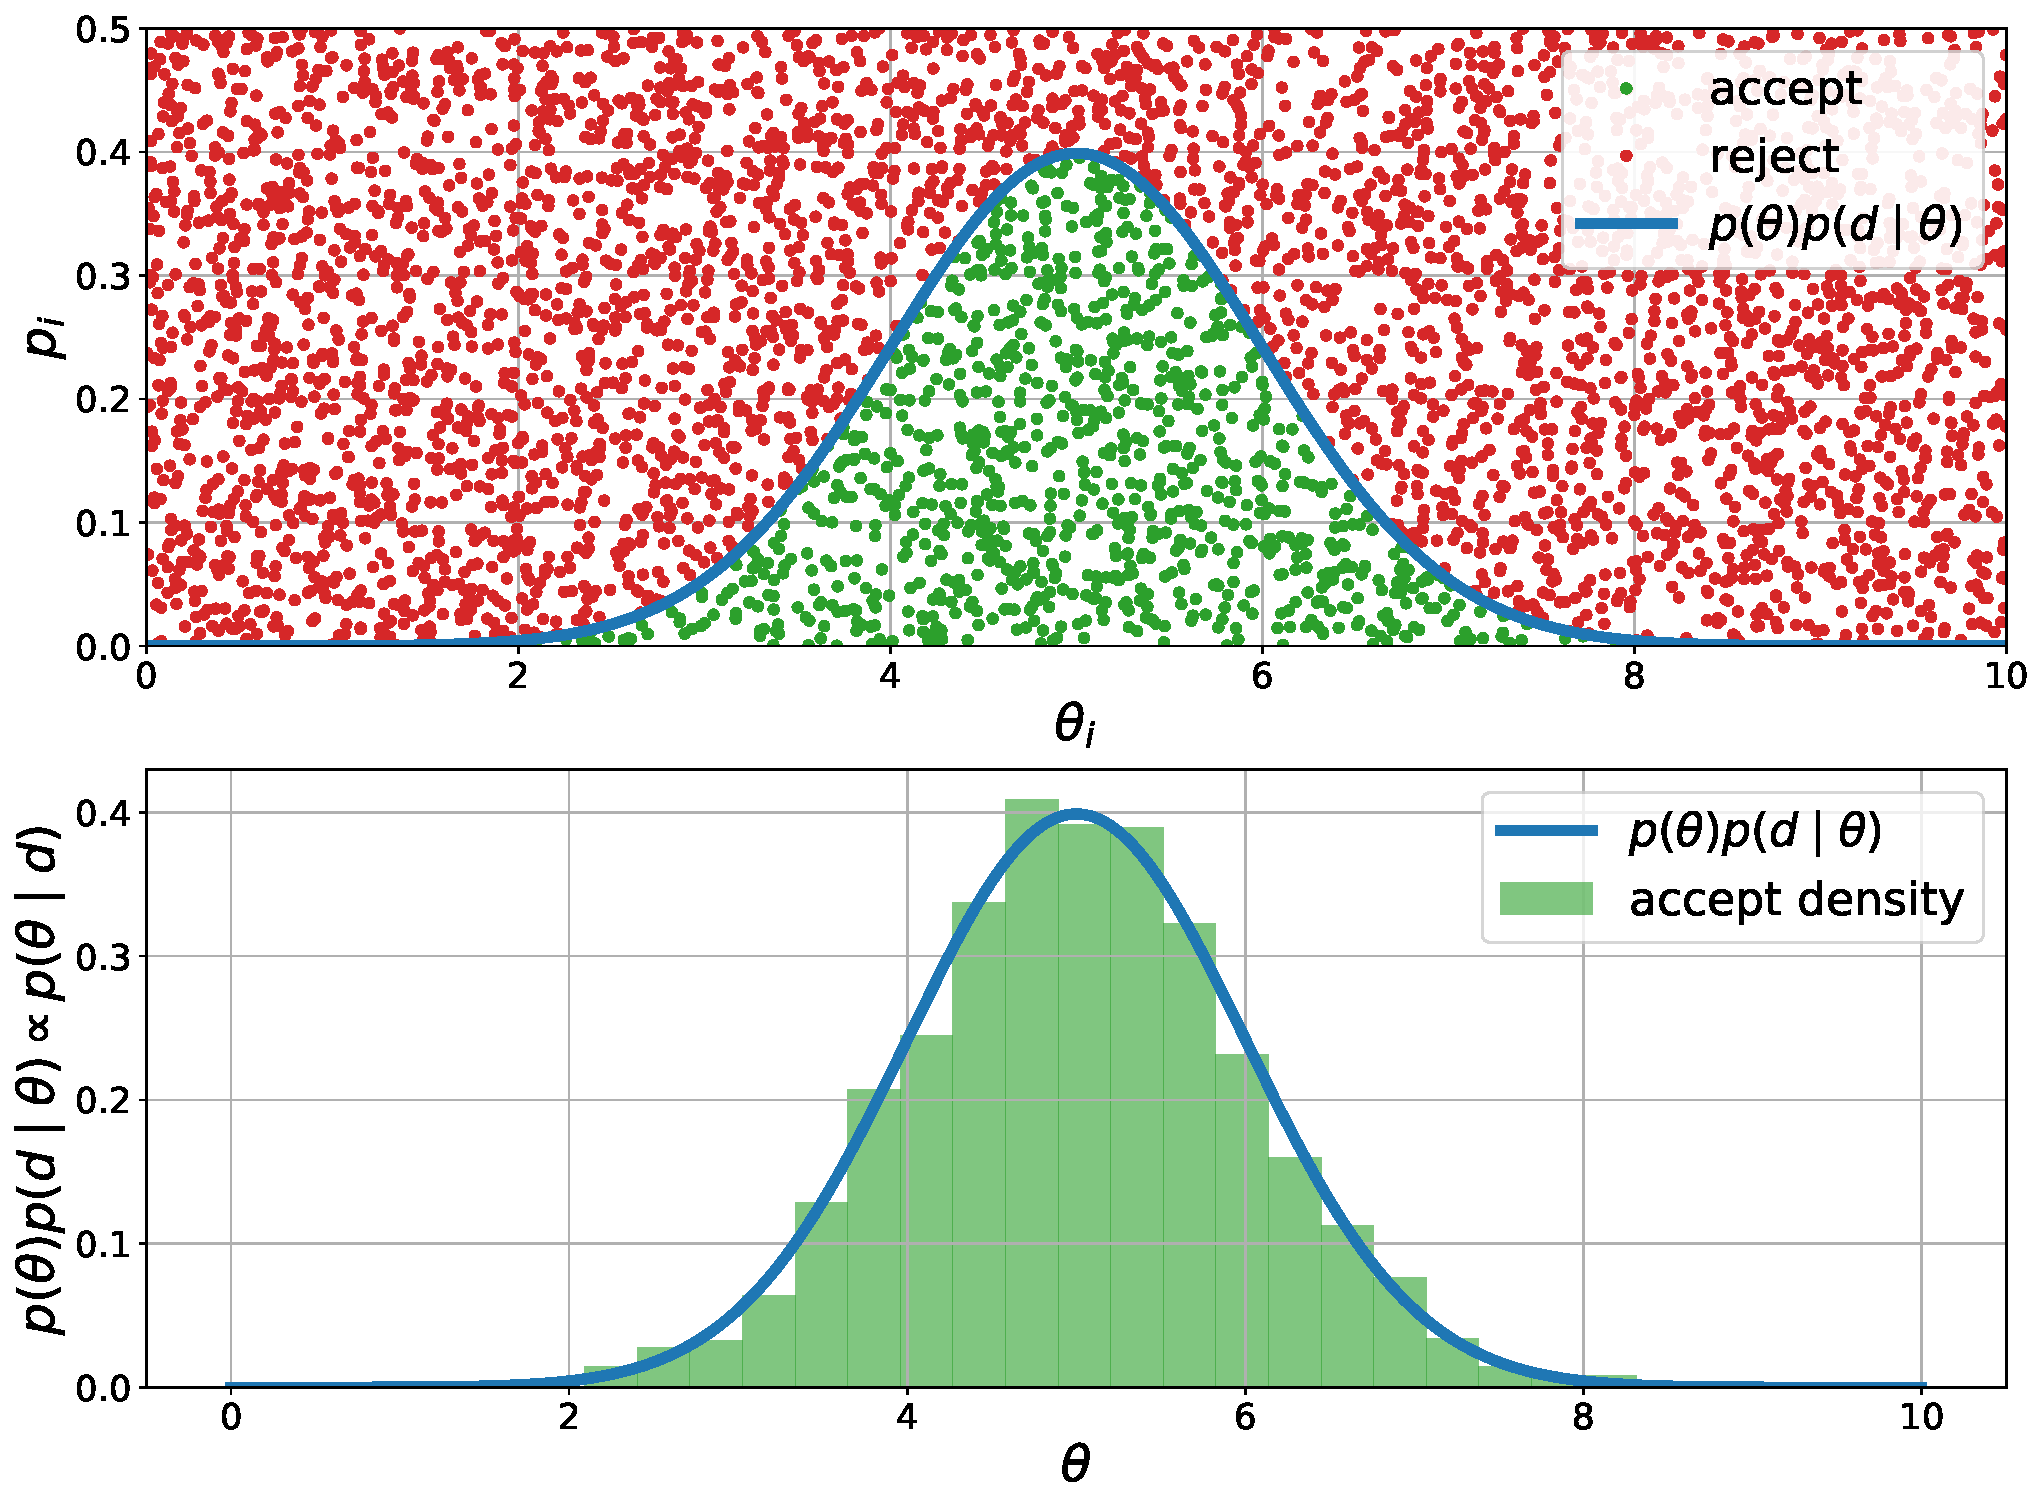
\includegraphics[width=0.8\linewidth]{C2_cw/reject_sample.pdf}
        \caption[Rejection sampling example]{Example of rejection sampling
applied to a simple one dimensional Gaussian distribution. To top panel shows a
number of samples $(\theta_i, p_i)$ with the true posterior $p(\theta)$
overlaid, where the green samples are accepted and red samples are rejected.
The bottom panel shows a histogram of the accepted samples, where each bin
contains the density of points in the range $\theta \rightarrow \theta + \delta
\theta$.} \label{cwinto:bayes:sampling:rejection}
\end{figure}
%

Whilst this method provides an easy way to understand sampling a distribution, it is computationally inefficient. For example, it is often the case that the posterior distribution $p(\theta \mid \bm{d})$ is narrow and covers a small area of parameter space, this method would then discard many more samples than it accepts, wasting computational time calculating the posterior value at these points. 
When there are a larger number of parameters $\left\{\theta^{(1)},\theta^{(2)}, ....\right\}$, rejection sampling can quickly become impractical due to the computational time required to estimate the posterior distribution of those parameters $p(\theta^{(1)},\theta^{(2)}, .... \mid \bm{d})$.
There are however other techniques which have been developed which can sample the posterior distribution more efficiently.

%
\subsubsection{MCMC}
%

As described in Sec.~\ref{searchcw:bayes:rejection}, rejection sampling is an inefficient method to sample from a posterior distribution, especially if the posterior is located in a small region of parameter space.
Therefore, another sampling method titled \gls{MCMC} can be used which concentrates the samples around areas of high probability,
approximating the posterior distribution more efficiently. More information on
this technique can be found in
\citep{metropolis1953EquationState,vanravenzwaaij2018SimpleIntroduction,sharma2017MarkovChain}.
Rather than calculating the posterior for many independent locations in
parameter space, an \gls{MCMC} algorithm randomly wanders around in parameter
space such that the amount of time spent in any location is proportional to the
height of the distribution.  An example of a simple \gls{MCMC} algorithm can be
seen in Alg.~\ref{searchcw:bayes:mcmc_alg}.

An \gls{MCMC} algorithm
builds up samples from the posterior distribution by using a Markov chain, where each
step in the chain only depends on the previous step.  
It starts by calculating the posterior value for a particular point in parameter space. Then it will
randomly jump to another point parameter space, where a new value for the
posterior can be calculated.  The size of the `jump' is defined by a proposal distribution (usually a Gaussian), which makes it difficult to jump to a value far away from the current value. If the new posterior value is higher than the
previous step then the jump is `accepted', which means that the parameter
values of this point are assumed to be from the posterior distribution and are recorded.  If the posterior value is lower than the
previous step then the jump is accepted with a probability which is the ratio of the probabilities at the new and old locations.
The probability of acceptance can be written as
\begin{equation}
\label{searchcw:bayes:mcmc:accept}
	p_{\rm{accept}} = 
	\begin{cases}
		\frac{p(\theta_i \mid \bm{d})}{p(\theta_{i-1} \mid \bm{d})} & \text{if} \; p(\theta_i \mid \bm{d}) < p(\theta_{i-1} \mid \bm{d}) \\
		1 & \text{if} \; p(\theta_i \mid \bm{d}) \geq p(\theta_{i-1} \mid \bm{d}) \\
	\end{cases},
\end{equation}
where $p(\theta_i \mid \bm{d})$ is the posterior value at the current parameter location and $p(\theta_{i-1} \mid \bm{d})$ is the posterior value at the previous parameter location. 
This means that the accepted positions are located around areas of high
posterior values, the \gls{MCMC} algorithm does not waste time calculating the
posterior in uninteresting areas of parameter space.  
One can see this correctly samples the posterior distribution by thinking about the condition in Eq.~\ref{searchcw:bayes:mcmc:accept}. Say we only allow jumps between two locations in parameter space, one which corresponds to the maximum of the posterior and one at half of this value. 
If we start at the maximum, the probability of accepting the jump to the parameter with half the value of the posterior is $0.5$. Repeating this many times would mean that the chain would jump to the lower value half the time, and therefore have half the samples at the parameter which is at half the maximum of the posterior. 
The accepted samples then have a density proportional to the posterior distribution. 
%
\begin{algorithm}
	\centering
	\begin{algorithmic}[1]
		\STATE{Input: N} \COMMENT{Chain length}
		\STATE{Output: S} \COMMENT{Samples}
		\STATE
		\STATE{Initialisation: $\theta_0$}
		
		\FOR{Sample, $i=1 \rightarrow N$}
			\STATE{$\theta_i = \theta_{i-1} + f$}
			\IF{$p(\theta_i \mid \bm{d}) > p(\theta_{i-1} \mid \bm{d})$ }
				\STATE{$S_i = \theta_i$}
			\ELSE
				\IF{$\frac{p(\theta_i \mid \bm{d})}{p(\theta_{i-1} \mid \bm{d})} < U(0,1)$ }
					\STATE{$S_i = \theta_i$}
				\ELSE
					\STATE{$S_i = \theta_{i-1}$}
				\ENDIF
		\ENDIF
		\ENDFOR
		\STATE

		%
	\end{algorithmic}
        \caption[Simple MCMC algorithm]{This is a basic pseudo MCMC algorithm,
where we draw samples $\theta_i$ from the posterior distribution $p(\theta_i
\mid \bm{d})$. Here $f$ is some distribution (often a Gaussian) which describes the jump
to the new point in parameter space and $U(0,1)$ is a values drawn from a
uniform distribution between 0 and 1. This algorithm returns a set of samples
$S$ from the posterior distribution $p(\theta_i \mid \bm{d})$.
\label{searchcw:bayes:mcmc_alg}}

\end{algorithm}

%
\subsubsection{\label{searchcw:prob:bayes:nested}Nested Sampling}
%


In Bayesian inference it is often useful to compare different models or hypotheses to gain insight into which is more likely. One can do this by using the Bayes
factor
%
\begin{equation}
B = \frac{p({\bm d} \mid I_1)}{p({\bm d} \mid I_2)},
\end{equation}
%
which compares the marginal likelihood of one model $p({\bm d} \mid I_1)$ to the marginal likelihood of another $p({\bm d} \mid I_2)$ and describes the evidence in favour of one model over the other.
This requires the calculation of the Bayesian Evidence in Eq.~\ref{searchcw:bayes:evidence}, which traditionally is very difficult to calculate as it is an integral over the entire parameter space. To calculate this, a method known as nested sampling was developed
\citep{skilling2006NestedSampling,speagle2019DynestyDynamic}.
In nested sampling, rather than directly sampling from the posterior as in \gls{MCMC}, the posterior is broken into `slices' where samples are generated from each `slice'.
The posterior is reconstructed by combining the samples using weights associated with each slice.
The idea is to transform the integral for the Bayesian Evidence such that it is no longer multidimensional.
This is done by using the prior mass, defined by
\begin{equation}
\label{searchcw:bayes:nested:priormass}
X(\lambda) = \int_{\theta: \mathcal{L}(\theta) > \lambda} \pi(\theta) d\theta,
\end{equation}
where $\pi(\theta) = p(\theta \mid I)$ is the prior and $\mathcal{L}(\theta)=p(\bm{d} \mid \theta, I)$ is the likelihood. This is the amount of the prior where the likelihood $\mathcal{L}(\theta)$ is greater than some value $\lambda$.
The Bayesian Evidence is then defined as 
\begin{equation}
\label{searchcw:bayes:nested:evidence}
Z = p(\bm{d} \mid I) = \int \mathcal{L}(\theta) \pi(\theta) d\theta = \int_0^1 \mathcal{L}(X) dX,
\end{equation}
where $\mathcal{L}(X)$ is the value of the likelihood where $P(\mathcal{L}(\theta) > \lambda) = X$. One can find how we can get to this integral in Appendix \ref{appb}.
The integral for the Bayesian Evidence has then been transformed to a one dimensional integral between 0 and 1 over the prior mass rather than a potentially multidimensional integral over $\theta$.

In Fig.~\ref{cwinto:bayes:nestedsampling:plots} the prior mass is shown for a
given value of $\lambda$ as the blue shaded area in the first panel, where this area is the amount of the prior in areas of parameter space where $\mathcal{L}(\theta) > \lambda$.
One can then see that when $\lambda= 0$ the prior mass must be one, and as $\lambda \rightarrow \infty$ the prior mass must approach zero. The bottom right panel of Fig.~\ref{cwinto:bayes:nestedsampling:plots} shows the equivalent plot where as the prior mass decreases, the value of the likelihood at that prior mass increases.
The two representations of the Bayesian Evidence defined in Eq.~\ref{searchcw:bayes:nested:evidence} can then be seen as the integral of the lower two panels in Fig.~\ref{cwinto:bayes:nestedsampling:plots} respectively, where the shaded regions represent $Z$. 
%
\begin{figure}[ht]
	\centering
	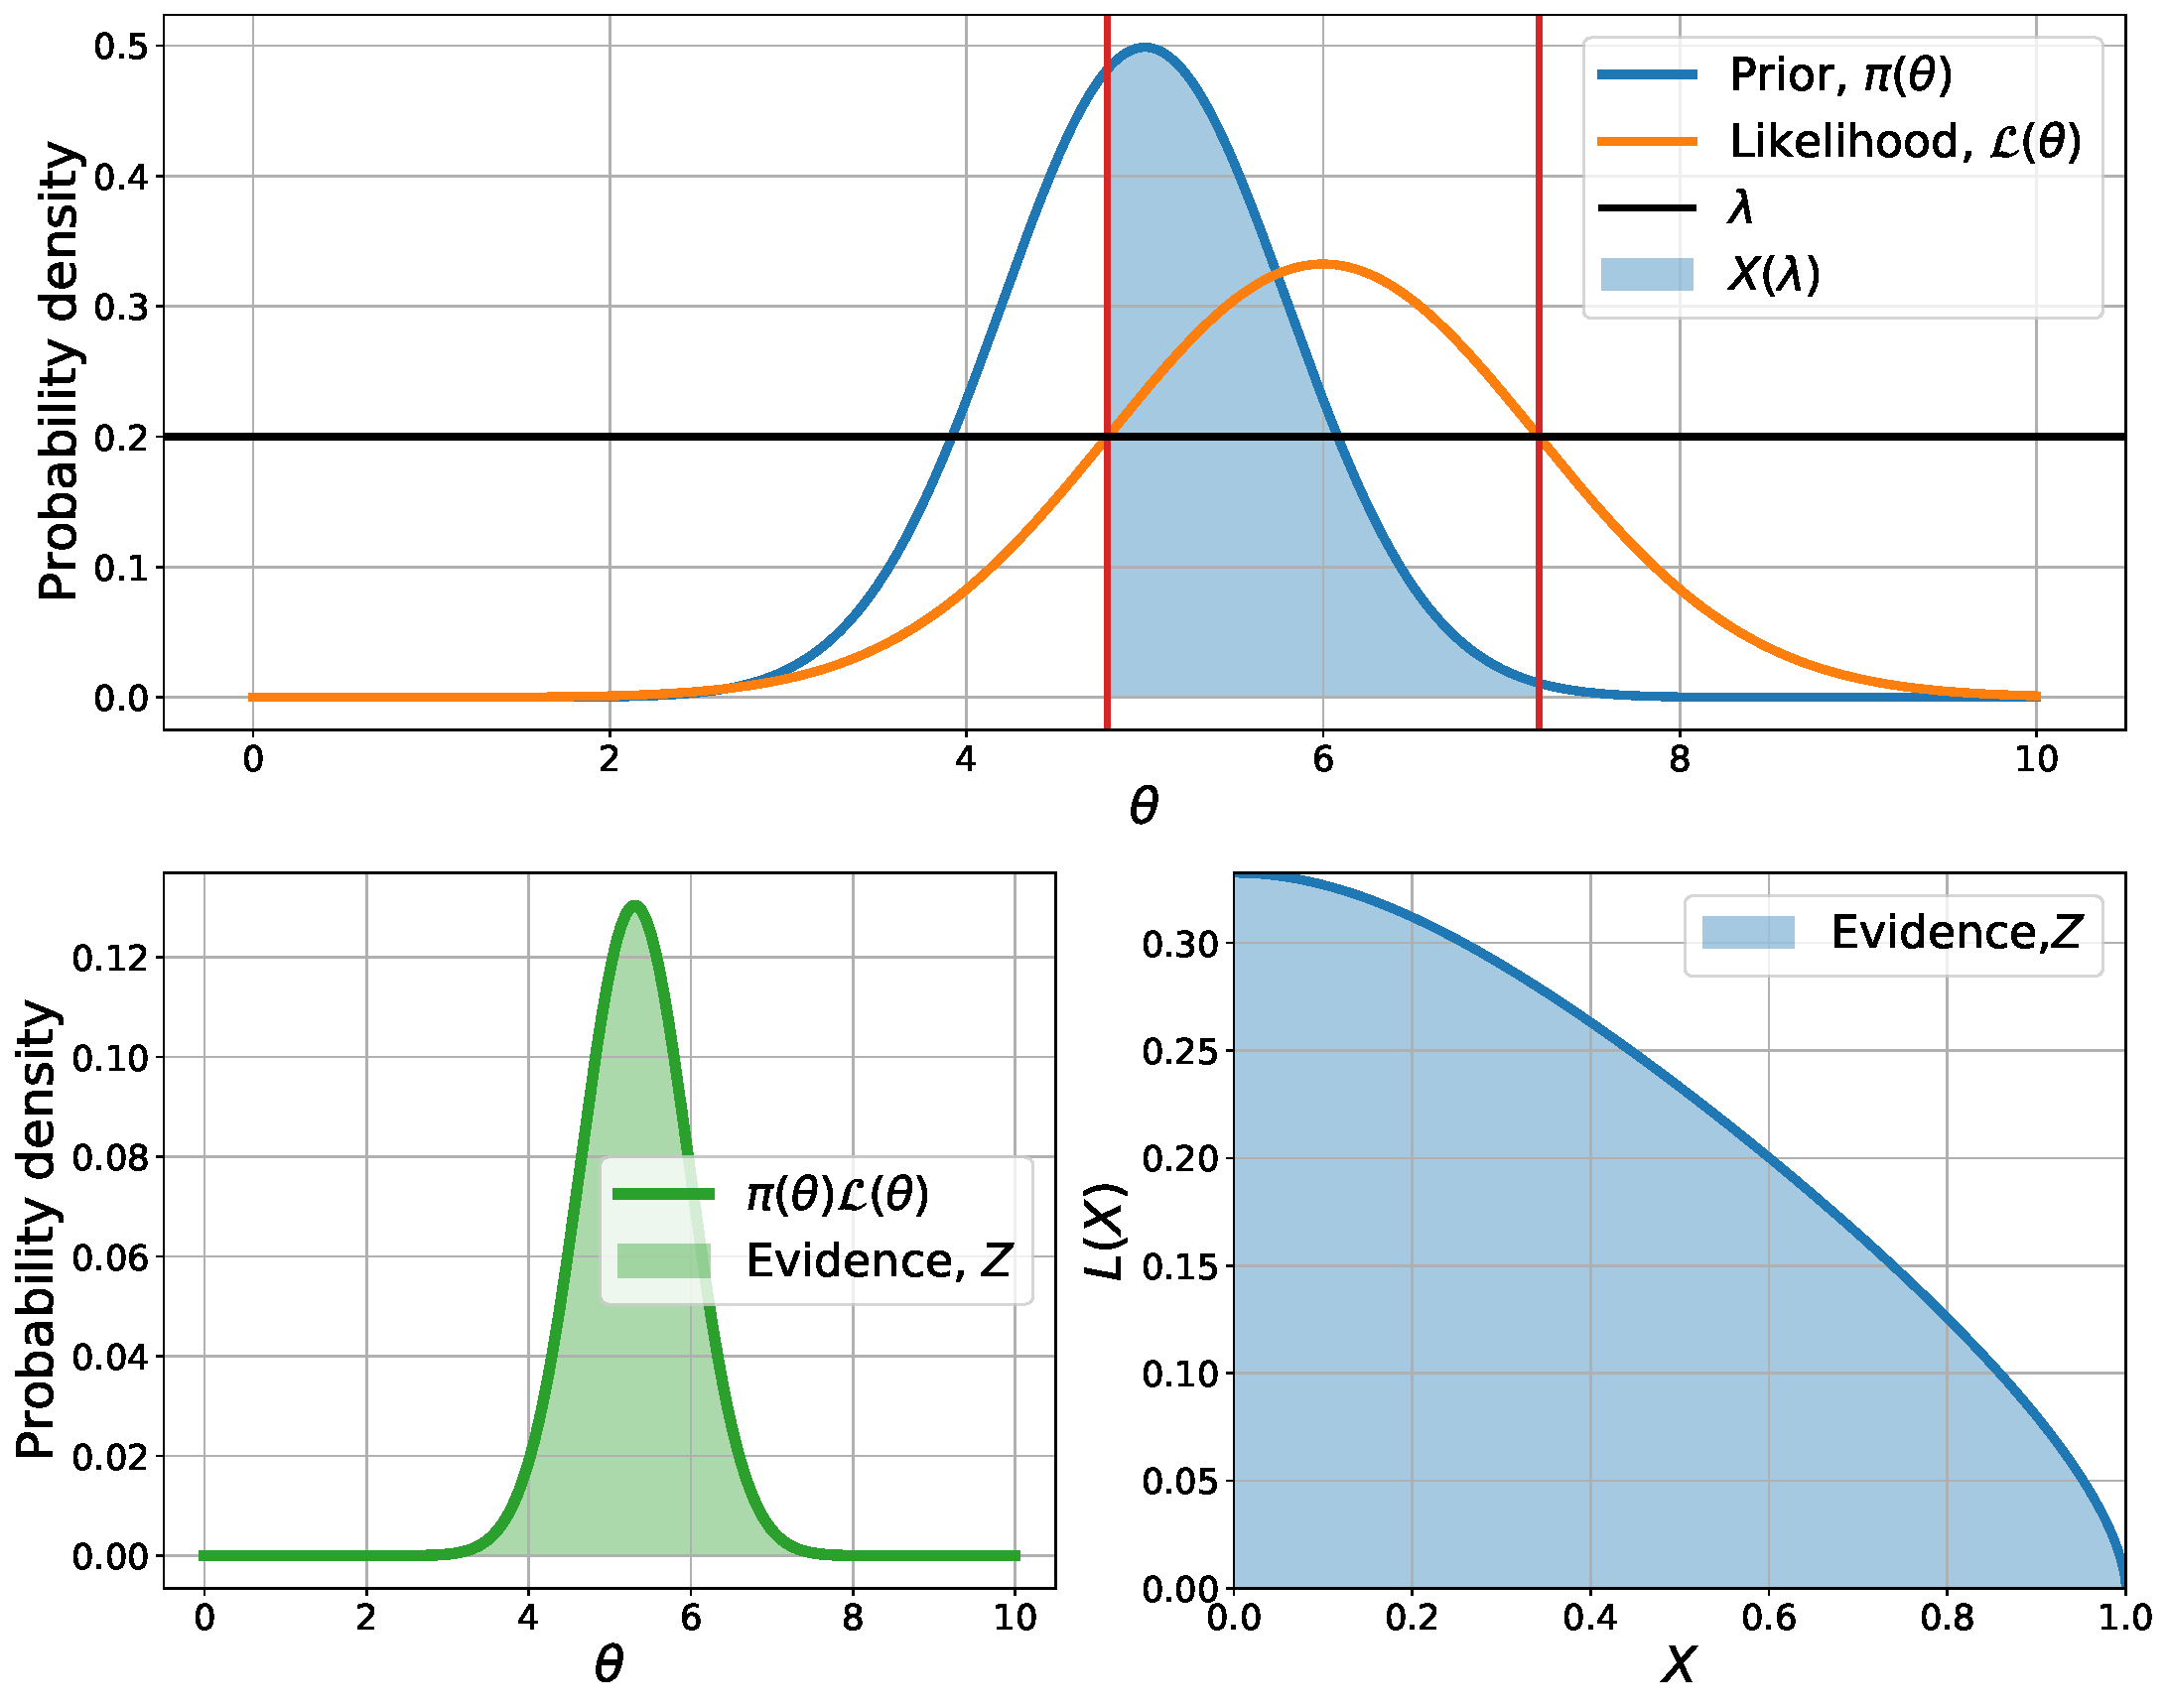
\includegraphics[width=0.8\linewidth]{C2_cw/nested_plots.pdf}
        \caption[Nested sampling]{An example of a prior distribution and a
likelihood are shown in the first panel for a 1D distribution, where the prior
mass $X(\lambda)$ is the shaded region for a given $\lambda$ defined in
Eq.~\ref{searchcw:bayes:nested:priormass}. The bottom left panel then shows
$\pi(\theta)\mathcal{L}(\theta)$, where the integral of this defined in
Eq.~\ref{searchcw:bayes:nested:evidence} is the Evidence $Z$. The bottom right
panel shows the likelihood as a function of prior mass which or any number of
parameters is a 1D integral, where again the integral of this is the Evidence
in Eq.~\ref{searchcw:bayes:nested:evidence}.}
\label{cwinto:bayes:nestedsampling:plots}

\end{figure}
%

If the form of $\mathcal{L}(X)$ is known, then the Evidence could be approximated numerically by evaluating $\mathcal{L}_i = \mathcal{L}(X_i)$ for a number of values of the prior mass $0 < X_M < ... < X_1 < X_0 = 1$ such that
\begin{equation}
\label{searchcw:bayes:nested:evidence_trapz}
Z \approx \hat{Z} = \sum_{i=1}^{M} \mathcal{L}_i \left[  X_{i-1} - X_{i}\right].
\end{equation} 
This would just be summing the area in columns under the curve in the bottom right panel of Fig.~\ref{cwinto:bayes:nestedsampling:plots}, however $\mathcal{L}(X)$  is typically not known.

Nested sampling algorithms instead estimate $Z$ by drawing samples from the constrained prior mass as described in Alg.~\ref{searchcw:bayes:nested_alg}.
One could take $N_{\rm{live}}$ samples (or live points) of $\theta$ from the prior distribution $\pi(\theta)$, then calculate the minimum value of the likelihood for these values $\mathcal{L}_{\rm{min}}$ and save the values of the parameters $\theta_{\rm{min}}$ associated with this likelihood.
The sample $\theta_{\rm{min}}$ can then be replaced with a new sample from the prior distribution with the constraint that $\mathcal{L}(\theta) > \mathcal{L}_{\rm{min}}$. This process can then be repeated a number $M$ times.
This then records samples $\theta_{\rm{min}}$ after each step such that the values of $\mathcal{L}_{\rm{min}}$ are increasing, and therefore $X$ is decreasing
\begin{equation}
	0 < X_M < ... < X_1 < X_0 = 1.
\end{equation}
The values of $\mathcal{L}_{\rm{min}}$ can then be used with Eq.~\ref{searchcw:bayes:nested:evidence_trapz} to approximate the evidence , where the prior mass would be calculated for each step $X_i = P(\mathcal{L}(\theta) > \mathcal{L}_{\rm{min},i})$.
However, we can notice that the value of the prior mass shrinks at each step following $X_i = t_i X_{i-1}$, where $t_i$ follows the distribution of the maximum value of $N_{\text{live}}$ samples from $U(0,1)$, i.e. $f(t) = N_{\text{live}} t^{N_{\text{live}} - 1}$.
Therefore, rather than calculating the prior pass at each stage, we can assume the prior mass is a random variable, where after each iteration it shrinks by the expectation value of $t_i$
\begin{equation}
E[t_i] \approx \exp{\left(-\frac{i}{N_{\rm{live}}}\right)},
\end{equation}
%
and then after each step we can set $X_i = E[t_i] X_{i-1}$ \citep{feroz2019ImportanceNested}.
This tells us that using this algorithm the log-prior mass shrinks by a factor $\sim -1/N_{\rm{live}}$ after each iteration \citep{speagle2019DynestyDynamic}. 

%
\begin{algorithm}
	\centering
	\begin{algorithmic}[1]
		\STATE{Draw $N_{\rm{live}}$ ``live'' points $\left\{ \theta_{n=1},...\theta_{N_{\rm{live}}} \right\}$ from the prior $\pi(\theta)$} \COMMENT{Samples from the prior distribution}
		
		\STATE{initialise: $D$} \COMMENT{initialise a list to store samples}
		\STATE{initialise: $Z = 0$} \COMMENT{Initialise the Evidence calculation}
		\STATE{initialise: $i=0$} \COMMENT{initialise a list to store samples}
		
		\WHILE{stopping criterion not met}
		\STATE{ $\mathcal{L}^{\rm{min}} = \rm{min}\left\{\mathcal{L}(\theta_1),...\mathcal{L}(\theta_{N_{\rm{live}}})\right\}$} \COMMENT{find minimum likelihood values for all live points}
		\STATE{$D_i  = \theta_n$ } \COMMENT{add the live point $\theta_n$ associated with $\mathcal{L}^{\rm{min}}$ to list of `dead' points $D$.}
		\STATE{draw $\theta_{\rm{new}}$ from constrained prior where $\mathcal{L}(\theta_{\rm{new}}) > \mathcal{L}^{\rm{min}}$}
		\STATE{$\theta_n = \theta_{\rm{new}}$}
		\STATE{$Z = Z +\mathcal{L}^{\rm{min}} \Delta X = Z + 1/N_{\rm{live}}$} \COMMENT{add point to the sum of the Evidence as Eq.~\ref{searchcw:bayes:nested:approx_evidence}}
		\STATE{Evaluate stopping criterion}
		\STATE{$i = i+1$}
		\ENDWHILE
		\STATE
		\STATE{Estimate the final part of the prior volume from remaining live points.}
		\WHILE{$N_{\rm{live}} > 0$}
			\STATE{$\mathcal{L}^{\rm{min}} = \rm{min}\left\{\mathcal{L}(\theta_1),...\mathcal{L}(\theta_{N_{\rm{live}}})\right\}$} \COMMENT{compute minimum likelihood of current live points}
			\STATE{$D_i  = \theta_n$ } \COMMENT{add the live point $\theta_n$ associated with $\mathcal{L}^{\rm{min}}$ to list of `dead' points $D$.}
			\STATE{remove $\theta_n$}
			\STATE{$N_{\rm{live}} = N_{\rm{live}} - 1$}
		\ENDWHILE
		\STATE
		
		%
	\end{algorithmic}
        \caption[Nested sampling algorithm]{ Nested sampling algorithm from
\citep{speagle2019DynestyDynamic}. This describes how the evidence integral in
Eq.~\ref{searchcw:bayes:nested:evidence} can be approximated by sampling over
increasingly smaller prior masses.  \label{searchcw:bayes:nested_alg}}
\end{algorithm}
%

The integral in Eq.~\ref{searchcw:bayes:nested:evidence} can then be approximated using Eq.~\ref{searchcw:bayes:nested:evidence_trapz},
\begin{equation}
\label{searchcw:bayes:nested:approx_evidence}
	Z = \int_0^1 \mathcal{L}(X) dX \approx \sum_{i=1}^{i=M}  \mathcal{L}(\theta_i)  \left[ X_{i-1} - X_{i} \right] = \sum_{i=1}^{M} p(\theta_i),
\end{equation}
where $M$ is the number of iterations in Alg.~\ref{searchcw:bayes:nested_alg}, $p(\theta_i)$ is the importance weight defined as $p(\theta_i) =  \mathcal{L}(\theta_i) \left[ X_{i-1} - X_{i} \right]$. The likelihood value $\mathcal{L}(\theta_i)$ is calculated for each dead point $D_i$ with its associated change in prior mass $\Delta X = \left[ X_{i-1} - X_{i} \right] \approx -1/K$. 
This then gives an estimate of the Bayesian Evidence, for more details on this and some simple examples see \citep{skilling2006NestedSampling,speagle2019DynestyDynamic,feroz2019ImportanceNested}.

Nested sampling also provides an estimate of the posterior distribution as well as the Bayesian Evidence, from the set of samples (dead points) 
\begin{equation}
	p(\theta \mid \bm{d}, I) \approx \frac{\sum_{i=1}^{M} p(\theta_i) \delta(\theta - \theta_i)}{\sum_{i=1}^{M} p(\theta_i) }.
\end{equation}
where $\delta( \theta - \theta_i)$ is the Dirac delta
function \citep{speagle2019DynestyDynamic}.~\chris{this is correct and leaves
you with a sea of delta functions. Are you able to say anything about what you
then do with these, i.e., histgram them?}

The methods described above then provide a way to estimate parameters of a
model given some data.  Also this provides a way to compare different models
given some observation.  In chapters \ref{soap}, \ref{machine} and
\ref{par_est} the methods described above are used to estimate various
parameters.

%%%%%%%%%%%
%%%%%%%%%%%%%
\section{\label{searchcw:search} Continuous wave searches}
%%%%%%%%%%%%%%%%%%
%%%%%%%%%%%%%%%%%%

Searches for \glspl{CW} can be split into three general categories: Targeted
searches, Directed searches and All-sky searches, where the different
categories are based on the number of source parameters for which there is an estimate of its value prior to running the search.

%%%%%%
%%%%%%
\subsection{\label{searchcw:search:targeted}Targeted}
%%%%%%
%%%%%%

Targeted searches are used to search for specific
pulsars which have parameters known from electromagnetic observations, i.e.
X-ray, radio or $\gamma$-ray.  These observations can give accurate estimates of the sky position parameters
$\alpha$ and $\delta$, and the source frequency parameters $f$ and its
derivatives, where there could also be extra parameters if the pulsar is in a
binary system.
Targeted searches can then use these parameters as input such that they search
over the remaining unknown parameters $h_0, \iota, \phi_0, \psi$.  The
main targeted searches are the Bayesian time-domain search
\citep{dupuis2005BayesianEstimation}, the matched filter
$\mathcal{F}$-statistic \citep{schutz1998DataAnalysis} and the 5-Vector
approach \citep{astone2010MethodDetection}.

The Bayesian time-domain takes advantage ot the narrow-band nature of the signal and reduces the dataset to a manageable size such that Bayesian parameter
estimation can be applied with a reasonable computational cost.  This search
uses sky position and frequency parameters of the source to perform a slowly
evolving heterodyne which removes the phase evolution of the signal
\citep{dupuis2005BayesianEstimation}.  This allows
the signal to be low pass filtered and heavily downsampled without losing any
of the signal information.  This reduced dataset can then be used in a Bayesian
approach to generate posterior distributions on the parameters $h_0, \iota, \phi_0, \psi$, see
\citep{dupuis2005BayesianEstimation} for further information.  

The matched filter $\mathcal{F}$-statistic \citep{schutz1998DataAnalysis} analytically maximises a likelihood ratio with respect to the neutron stars amplitude parameters $h_0, \iota, \phi_0, \psi$ such that it then only a function of the Doppler parameters $\alpha, \delta, f$ and $\dot{f}$. 
This method resamples the data over some time length $T_{\rm coh}$ based on the parameters $\alpha, \delta, f$ and $\dot{f}$ using the \gls{SSB} time in Eq.~\ref{searchcw:model:ssbtime} \citep{schutz1998DataAnalysis}.
If the \gls{GW} signal matches these parameters then resampling removes the Doppler modulation of the signal such that it appears at a fixed frequency.
This means that the $\mathcal{F}$-statistic can be efficiently calculated using the \gls{FFT}. 
Once the maximum of the $\mathcal{F}$-statistic with respect to parameters $\alpha, \delta, f$ and $\dot{f}$  is found, the amplitude parameters can be analytically calculated from these parameters.
For more details on this search see \citep{schutz1998DataAnalysis,brady2000SearchingPeriodic,prix2007SearchContinuous,
aasi2014GRAVITATIONALWAVES}.

The 5-Vector search is based in the frequency domain, where it makes
use of the five frequency harmonics caused by the sidereal amplitude
modulation which originates from the detectors antenna response as
the earth rotates \citep{astone2010MethodDetection,aasi2014GRAVITATIONALWAVES}.
A summary of the application of these three searches for initial and advanced
\gls{LIGO} can be found in
\citep{aasi2014GRAVITATIONALWAVES,abbott2019SearchesGravitationala}.

Due to the long observation times needed to accumulate the required \gls{SNR}
for detection, most searches use data from an entire or multiple \gls{LIGO} and Virgo observing runs
which can last for $\mathcal{O}(1)$ year.  Given
that the sampling rate for the \gls{GW} channel is $16$ kHz (often downsampled
to $\sim 4$ kHz), the amount of data in a year can be $\mathcal{O}(2)$
terabytes, therefore these types of search can be computationally costly.
Whilst the fully coherent matched filter searches have methods to reduce the
computational time for known sources, in wide parameter space searches such as all-sky and directed searches, this
type of search is not feasible. 
This is due to the computational cost associated with running a fully coherent search over a wide parameter space.
This problem led to the development of semi-coherent searches which will be introduced in the
next sections. 

%%%%%%
%%%%%%
\subsection{\label{searchcw:search:directed}Directed}
%%%%%%
%%%%%%

In directed searches, the sky position parameters
$(\alpha,\delta)$ are known but the rotation frequency and other parameters are not. 
This includes searches for neutron stars in binary systems such as Sco-X1
\citep{abbott2017UpperLimits,meadors2016TuningScorpius}, for young supernovae remnants \citep{abadie2010FIRSTSEARCH} and for neutron stars in the galactic center \citep{piccinni2019DirectedSearch}. These searches use similar techniques as all-sky searches, which will be described in
Sec.~\ref{searchcw:search:allsky}, they differ in that they can limit the
parameter space based on the known sky position.

%%%%%%
%%%%%%
\subsection{\label{searchcw:search:allsky}All-sky searches}
%%%%%%
%%%%%%

All-sky searches have no prior knowledge of the pulsars parameters, therefore,
they are used to search over all the neutron star parameters $h_0, \iota, \psi, \phi_0, f,
\dot{f}, \alpha, \delta$. It would not be feasible to use the techniques described in
Sec.~\ref{searchcw:search:targeted} for an all sky search as to sufficiently
cover the entire parameter space, it would require large computational cost.  Instead
semi-coherent searches were developed.  These offered a solution to searching over
the large parameter space and data size.  The general idea of a semi-coherent
search is to break the dataset into smaller segments of length $T_{coh}$, which
can each be analysed coherently. There are also searches such as \citep{messenger2007FastSearch}, which breaks the dataset into smaller frequency bands and combined them incoherently. 
The results from each segment can the be combined incoherently using various methods which will be
summarised below.  
Whilst these methods will be less sensitive than a fully coherent search, they are much faster and at a fixed computing cost are more sensitive.

There are many different types of semi-coherent search which use various
methods to incoherently combine the coherently analysed time segments.  Some of these methods are summarised and compared in
\citep{walsh2016ComparisonMethods} and I will summarise these and others below.


\begin{description}
	
        \item[Stack-slide] This method uses a set of Fourier
transforms of the data known as \glspl{SFT}, more specifically it uses their power
spectrum, i.e. $|S|^2$ where $S$ is the \gls{SFT}. Each of the separate
\glspl{SFT} (segments) is shifted up or down in frequency relative
to the others based on the sky position $\alpha$ and $\delta$ to account for the Doppler modulation of the source. The \gls{SFT}
power from each frequency bin can then be summed (stacked). More explanation of this can be found in
\citep{brady2000SearchingPeriodic, cutler2005ImprovedStackslide}  
	
        \item[Hough] The Hough transform is similar to the stack-slide algorithm.
The main difference is that the detection statistic for each segment is
assigned a weight of 0 or 1 depending if it crossed a detection threshold. These weighted set of \glspl{SFT} are then used as input to the Hough transform.
The Hough transform maps a pattern in an image such as a straight line ($y=mx + c$) to the parameters ($m,c$) which are consistent with that line.
This approach is explained in greater detail in
\citep{krishnan2004HoughTransform,antonucci2008DetectionPeriodic}.  This method
has been applied in two main ways known as Sky Hough
\citep{krishnan2004HoughTransform}, which generates Hough maps in sky position $(\alpha,\delta)$ for fixed spin down, and Frequency Hough
\citep{antonucci2008DetectionPeriodic,astone2014MethodAllsky} which generates hough maps in $(f,\dot{f})$ for fixed sky position.
	
        \item[Einstein@Home] \joe{reread this }This uses the
$\mathcal{F}$-statistic mentioned in Sec.~\ref{searchcw:search:targeted} calculated over a length of $T_{\rm{coh}}$, where in the initial stages of this search these segments are combined incoherently. This is is done using a Hough transform scheme \citep{theligoscientificcollaborationandthevirgocollaboration2013EinsteinHome} or by generating candidate events where the $\mathcal{F}$-statistic crosses some threshold and then finding events which are coincident in parameter space \citep{ligoscientificcollaboration2009EinsteinHome}.
After the first stage, potential signals are returned (candidates) where post processing methods as in \citep{theligoscientificcollaborationandthevirgocollaboration2013EinsteinHome} select the most significant candidates.
In \citep{theligoscientificcollaborationandthevirgocollaboration2013EinsteinHome} they use a three step procedure, which starts with the Hough transform with more finely sampled parameters around the candidate, and then runs a semi and then finally fully coherent $\mathcal{F}$-statistic analysis.
Other methods for combining results and following up candidates can be found in \citep{singh2016ResultsAllsky,papa2016HierarchicalFollowup,walsh2016ComparisonMethods}.
Einstein@Home is the most sensitive of the current all-sky \gls{CW} searches,
however, uses a large amount of computing power. This is possible due to the use of a
distributed computing project, where more details can be found at
\citep{EinsteinHome}. 
	
        \item[Time domain $\mathcal{F}$-statistic] The time domain
$\mathcal{F}$-statistic splits the data into narrowband segments of length
$\sim$ 2 days \citep{walsh2016ComparisonMethods}. Then a coherent search using
the $\mathcal{F}$-statistic is applied to each of these segments. Values of
this statistic above a threshold are stored. Coincidences are then found in
each segment, where candidates are selected best based on a given
threshold. This is explained in greater detail in
\citep{aasi2014ImplementationTextdollar,walsh2016ComparisonMethods}.
	
        \item[Powerflux] Powerflux uses a standard set of 1800s \glspl{SFT}.
For each point in parameter space, the frequency of a signal with those parameters is found and the power in each \gls{SFT} at that frequency is recorded. This power is then weighted depending on the antenna pattern and
noise of the detector. In longer stretches of $\sim$ 1 month, the weighted
power is summed. Any point in parameter space which produces high power in each
of these stretches is identified as a potential signal. This search can then be
repeated around each candidate with a finer resolution in parameter space. This
is explained in more detail and tested in
\citep{abadie2012AllskySearch,walsh2016ComparisonMethods,ligoscientificcollaborationandvirgocollaboration2016ComprehensiveAllsky}
	
        \item[Viterbi] The Viterbi algorithm \citep{viterbi1967ErrorBounds} has
been used in \citep{sun2018HiddenMarkov,
suvorova2017HiddenMarkov,abbott2017SearchGravitational,
abbott2018SearchGravitational, sun2018ApplicationHidden} to search for a
\glspl{CW} with unknown randomly wandering spin frequency. This
algorithm was applied to specific sources, where the $\mathcal{F}$-statistic is
used on short duration segments which are then incoherently combined using the
Viterbi algorithm.
	
\end{description}

Each of these searches has a large computational cost. In \citep{walsh2016ComparisonMethods} a
\gls{MDC} was conducted to compare the sensitivity of some of the all-sky 
searches, where an expected runtime was presented for a search through the first four months of the first observing run of advanced \gls{LIGO} (O1), shown in Tab.~\ref{searchcw:search:semi:cost}. 
The results from O1 for some of these searches can be found in \citep{ligoscientificcollaborationandvirgocollaboration2017AllskySearch}.  
%
\begin{table}
	\centering
	%
        \caption[Computational cost of \gls{CW} searches.]{From
\citep{walsh2016ComparisonMethods}, shows the expected computational cost for the first
four months of the first observing run of advanced \gls{LIGO} (O1) for each search. This is measured in \glspl{MSU}, where one
standard unit is equal to one core-hour on a standard core.
The Einstein@Home searches uses the computing resources
of the Einstein@Home project and is designed to run for 6 - 10 months in the
Einstein@Home grid.
  \label{searchcw:search:semi:cost}}
	
	%
        \bgroup \def\arraystretch{1.5} \centering \begin{tabular}{|c c|} \hline
Pipeline & Expected runtime of O1 search \\ \hline Powerflux & 6.8 MSU \\

		Time domain $\mathcal{F}$-statistic & 1.6 MSU\\

		Frequency Hough & 0.9 MSU \\

		Sky Hough & 0.9 MSU\\
		\hline
		Einstein@Home & 100-170 MSU\\
		\hline

	\end{tabular}
	\egroup
\end{table}
%
Even the fastest of these searches takes close to 1 million core-hours to
search through four months of data. 
This presents one of the larger issues when searching for sources of \gls{CW} as generating results from observing runs can be time consuming. 


